
\documentclass[12pt,letterpaper]{article}


\usepackage[top=1in, 
		    bottom=1in,
		    left=1in,
		    right=1in]{geometry}
\usepackage{setspace}	% makes the \singlespacing, \onehalfspacing, and \doublespacing commands available
% \usepackage[en-US]{datetime2}
% \DTMlangsetup{showdayofmonth=false}
% \usepackage{titlesec}
\usepackage{listings}	% allows for placing programming code to be displayed correctly
\usepackage{siunitx}	% units
\usepackage{amsmath}
\usepackage{amsfonts}
\usepackage{amssymb}
\usepackage{graphicx}
\usepackage{booktabs}
\usepackage{multirow}
\usepackage{pgfplots}
\pgfplotsset{compat=newest}
\usepackage{tikz}
%\usetikzlibrary{shapes.geometric}
% \usepgfplotslibrary{external} 
% \tikzexternalize[prefix=pdfimages/,
% 		        mode=list and make]
\usepackage{caption}
\usepackage[list=true,
		     listformat=simple]{subcaption}
%\usepackage{cleveref}	% this should really go last
% \usepackage[colorlinks,
% 		     linkcolor=black,
% 		     citecolor=black,
% 		     plainpages=false,
% 		     pdfpagelabels]{hyperref}
% \usepackage[all]{hypcap}
\usepackage{cleveref}
% \doublespacing

\pagenumbering{gobble}
\newcommand{\mymder}[2]{\ensuremath{\frac{\mathrm{D}#1}{\mathrm{D}#2}}}
\newcommand{\mypder}[2]{\ensuremath{\frac{\partial #1}{\partial #2}}}
\newcommand{\mypdertwo}[2]{\ensuremath{\frac{\partial^2 #1}{\partial #2^2}}}
\newcommand{\mymdervec}[1]{\ensuremath{mypder{#1}{t} + }}
\newcommand{\myder}[2]{\ensuremath{\frac{d#1}{d#2}}}
\newcommand{\mydiv}[1]{\ensuremath{\nabla \cdot {#1}}}
\newcommand{\myfrac}[2]{\ensuremath{^{#1}\!/_{#2}}}
\newcommand{\myfunc}[2]{\ensuremath{#1 \left( #2 \right)}}
\newcommand{\myparen}[1]{\ensuremath{\left( #1 \right)}}
\newcommand{\mybrack}[1]{\ensuremath{\left[ #1 \right]}}
\newcommand{\mybrace}[1]{\ensuremath{\left\{ #1 \right\}}}
\newcommand{\mysin}[1]{\ensuremath{\myfunc{\mathrm{sin}}{#1}}}
\newcommand{\mycos}[1]{\ensuremath{\myfunc{\mathrm{cos}}{#1}}}
\newcommand{\myexp}[1]{\ensuremath{\myfunc{\mathrm{exp}}{#1}}}
\newcommand{\myint}[4]{\ensuremath{\int_{#1}^{#2} {#3} d {#4}}}


\newcommand{\Rld}{\ensuremath{\mathit{Re}}}
\newcommand{\St}{\ensuremath{\mathit{St}}}
\newcommand{\Prn}{\ensuremath{\mathit{Pr}}}
\newcommand{\Sc}{\ensuremath{\mathit{Sc}}}
\newcommand{\Sh}{\ensuremath{\mathit{Sh}}}
\newcommand{\Nu}{\ensuremath{\mathit{Nu}}}
\newcommand{\Bi}{\ensuremath{\mathit{Bi}}}


\let\textacute\'
\let\textgrave\`


\newcommand{\includetikz}[2]{%
    \tikzsetnextfilename{#2}%
    \input{#1#2.tex}%
}

\begin{document}

\noindent
MECH 131A Midterm Project

\noindent
Assigned date: November $3^{\mathrm{th}}$, 2024

\noindent
Due date: November $17^{\mathrm{th}}$, 2024

\subsubsection*{Instructions}
\begin{enumerate}
	\item This is a project for up to three people.
	\item If using a specific solution methodology is specified, please include a copy of the Python/MATLAB script.
	\item If using a specific solution methodology is \textit{not} specified, please include a copy of your computational methodology.
\end{enumerate}

\subsubsection*{Green House}

You retired from the rat race and want to buy some land and grow plants and tend some entitled chickens.
You decide to design a green house and want to estimate the daily and annual temperature variation within the green house.
Since no money is of no object when you are dreaming, you are trying to pick between low iron glass, high iron glass, fuzed quartz, and lucite.
For this analysis you can assume a cube shaped green house with the roof and south facing wall are glass, while the others are completely reflective of light.

\begin{enumerate}
    \item Draw a diagram showing \textit{all} the heat transfers for the green house.

    \item Describe the heat transfer correlations used for all the interior and exterior surfaces.

    \item Calculate the ratio of energy from sunlight that is reflected, transmitted and absorbed by each type of glass as a rough function of wavelength.
    
    \item For the summer and winter solstice, find the daily temperature variation from midnight to midnight.
        Find the temperature variation for each type of ``glass'' for 16 combinations of the following boundary conditions:
        \begin{enumerate}
            \item 0 \si{\meter\per\second} and 10 \si{\meter\per\second} for wind speed,
            \item \SI{235}{\kelvin} and \SI{285}{\kelvin} for the sky temperature,
            \item rain or no rain,
            \item and sunlight or no sunlight.
        \end{enumerate}
        Do any of the conditions seem to be more important than the others?
        Which combinations of the bounding assumptions are unlikely?
        To simplify the analysis you can assume 15 and 9 hours of daylight for the summer solstice and winter solstice, respectively.
        Further, you can assume a cosine function for the maximum irradiance of 1000 and \SI{800}{\watt\per\square\meter} for the summer and winter solstice, respectively
    
        \item How does the size of the cube affect the temperature variation?
            Give a brief explanation.
\end{enumerate}


\subsubsection*{Cryogenic Tank Heat Transfer}

You are part of a team that analyzes cryogenic propellant tank temperatures and pressures for a rocket.
Your team maintains a thermal lumped parameter model used to predict tank conditions throughout flight.
There is concern about the effect of the heat loss through wall of the tank near the top where the gas is (commonly called ``the ullage'').
Your task is to develop a model to more accurately predict the net heat transfer to the vehicle.
Currently, the model is lumped and assumes the walls temperature distribution is not important.
For the analysis below, you can assume the heat transfer coefficients for a given volume of fluid are the same at a wall-fluid interface and that radiative heat transfer within the tank is negligible.
There are three sets of bounding assumptions you will need to work with: wind speed, sky temperature, and cloud conditions.
The bounding assumptions are all eight combinations of 0 \si{\meter\per\second} and 10 \si{\meter\per\second} for wind speed, \SI{235}{\kelvin} and \SI{285}{\kelvin} for the sky temperature, and sunlight or no sunlight.

\begin{enumerate}
    \item Solve for the heat transfer in the default lumped model assuming the propellant are at saturation temperature.
    
    \item Derive the governing equation for the thin walls shown in the figure below.
        Assume you can ignore the transverse temperature change across the tank walls.
        Describe the two possible far-field boundary conditions for the tank walls in terms of the heat transfer coefficients.

    \item Describe the heat transfer correlations used for all the surfaces.

    \item Solve the inter-linked system of ordinary differential equations for all eight combinations of bounding assumptions.
        Comment on the effect of the wind speed, sky temperature, and sun visibility on the solution.
        Which combination of bounding is unlikely?

    \item Comment on how changing the height of the ullage affects the heat transfer to the ullage.
        Is there an optimum height to minimize the heat transfer to the ullage?

    \item The default model does not include correlation information or spatially changing wall temperatures.
        Comment on the differences of the more detailed model compared to the simple default model.
        What further improvements could you make if your manager wanted more accurate temperature and heat transfer predictions?
\end{enumerate}

\begin{figure}[!htpb]
	\centering
	% https://cremeronline.com/LaTeX/minimaltikz.pdf is a great primer for tikz

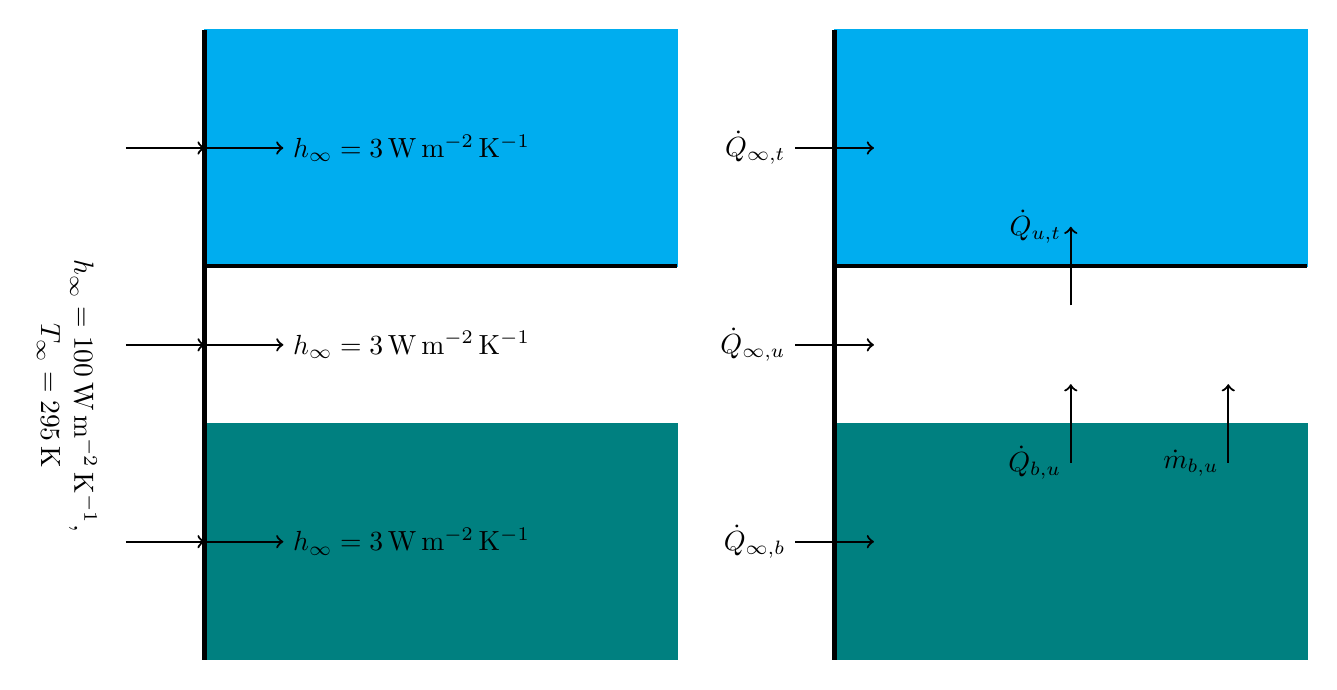
\begin{tikzpicture}
    %%  Draw Tank with htc Labels
    % Draw Tank
    \draw [fill=teal, draw=teal] (0,0) rectangle (6, -3);
    \draw [fill=cyan, draw=cyan] (0,2) rectangle (6,5);
    
    \draw [ultra thick] (0, -3) -- (0, 5);
    \draw [ultra thick] (0, 2) -- (6, 2);

    % Heat Transfer Coefficients
    \draw [->, thick] (-1, -1.5) -- (0, -1.5);
    \draw [->, thick] (-1, 1) -- (0, 1);
    \draw [->, thick] (-1, 3.5) -- (0, 3.5);
    \node [align=center, left, rotate=-90] at (-1.75, -1.5) {$h_{\infty} = \SI{100}{\watt\per\square\meter\per\kelvin}$, \\ $T_{\infty} = \SI{295}{\kelvin}$};
%    % Ambient to tank wall (bottom propellant)
%	\draw [->, thick] (-1, -1.5) -- (0, -1.5);
%    \node [align=center, left] at (-1, -1.5) {$h_{\infty} = \numrange{10}{100}~\si{\watt\per\square\meter\per\kelvin}$, \\ $T_{\infty} = \SI{295}{\kelvin}$};
%   % Ambient to tank wall (ullage propellant)
%	\draw [->, thick] (-1, 1) -- (0, 1);
%    \node [align=center, left] at (-1, 1) {$h_{\infty} = \numrange{10}{100}~\si{\watt\per\square\meter\per\kelvin}$, \\ $T_{\infty} = \SI{295}{\kelvin}$};
%    % Ambient to tank wall (top propellant)
%    \draw [->, thick] (-1, 3.5) -- (0, 3.5);
%    \node [align=center, left] at (-1, 3.5) {$h_{\infty} = \numrange{10}{100}~\si{\watt\per\square\meter\per\kelvin}$, \\ $T_{\infty} = \SI{295}{\kelvin}$};
    % Tank wall to bottom propellant
    \draw [->, thick] (0, -1.5) -- (1, -1.5);
    \node [align=center, right] at (1, -1.5) {$h_{\infty} = \SI{3}{\watt\per\square\meter\per\kelvin}$};
    % Tank wall to ullage
    \draw [->, thick] (0, 1) -- (1, 1);
    \node [align=center, right] at (1, 1) {$h_{\infty} = \SI{3}{\watt\per\square\meter\per\kelvin}$};
    % Tank wall to top propellant
    \draw [->, thick] (0, 3.5) -- (1, 3.5);
    \node [align=center, right] at (1, 3.5) {$h_{\infty} = \SI{3}{\watt\per\square\meter\per\kelvin}$};
    
   
    %%  Draw Tank with HT labels
    % Draw Tank
    \draw [fill=teal, draw=teal] (8,0) rectangle (14, -3);
    \draw [fill=cyan, draw=cyan] (8,2) rectangle (14,5);
    
    \draw [ultra thick] (8, -3) -- (8, 5);
    \draw [ultra thick] (8, 2) -- (14, 2);
    
    % HT
    % Ambient to bottom propellant
    \draw [->, thick] (7.5, -1.5) -- (8.5, -1.5);
    \node [left] at (7.5, -1.5) {$\dot{Q}_{\infty, b}$};
    % Ambient to ullage
    \draw [->, thick] (7.5, 1) -- (8.5, 1);
    \node [left] at (7.5, 1) {$\dot{Q}_{\infty, u}$};
    % Ambient to top propellant
    \draw [->, thick] (7.5, 3.5) -- (8.5, 3.5);
    \node [left] at (7.5, 3.5) {$\dot{Q}_{\infty, t}$};
    % Bottom propellant to ullage
    \draw [->, thick] (11, -0.5) -- (11, 0.5);
    \node [left] at (11, -0.5) {$\dot{Q}_{b, u}$};
    \draw [->, thick] (13, -0.5) -- (13, 0.5);
    \node [left] at (13, -0.5) {$\dot{m}_{b, u}$};
    % Ullage to top propellant
    \draw [->, thick] (11, 1.5) -- (11, 2.5);
    \node [left] at (11, 2.5) {$\dot{Q}_{u, t}$};
    
\end{tikzpicture}
	\caption{The figure on the left shows the expected ranges for the heat transfer coefficient when the there is \textit{no} boiling on the inside walls of the tank.
		The figure on the right shows all the heat transfers currently accounted for in the thermal model.
		If you need dimensional values for the tank, use the Saturn V second stage (S-II) which is \SI{10}{\meter} in diameter and had a hydrogen-LOX propellant mixture.
		You can assume the hydrogen and LOX are saturated at ambient conditions for this analysis.
		Further, and all though not pictured, there is a small vent in the tank that maintains the ullage pressure at ambient conditions.}
\end{figure}


\end{document}
